\documentclass{article}

\usepackage{graphicx}
\usepackage{tikz}
\usepackage{tikzsymbols}
\usetikzlibrary{calc,patterns,shapes.geometric}
\pagestyle{empty}
\usepackage[margin=0pt]{geometry}
\geometry{papersize={14in,12in}}

\def\centerarc[#1](#2)(#3:#4:#5){\draw[#1] ($(#2)+({#5*cos(#3)},{#5*sin(#3)})$) arc (#3:#4:#5);}

\begin{document}
	\begin{figure}
		\centering
		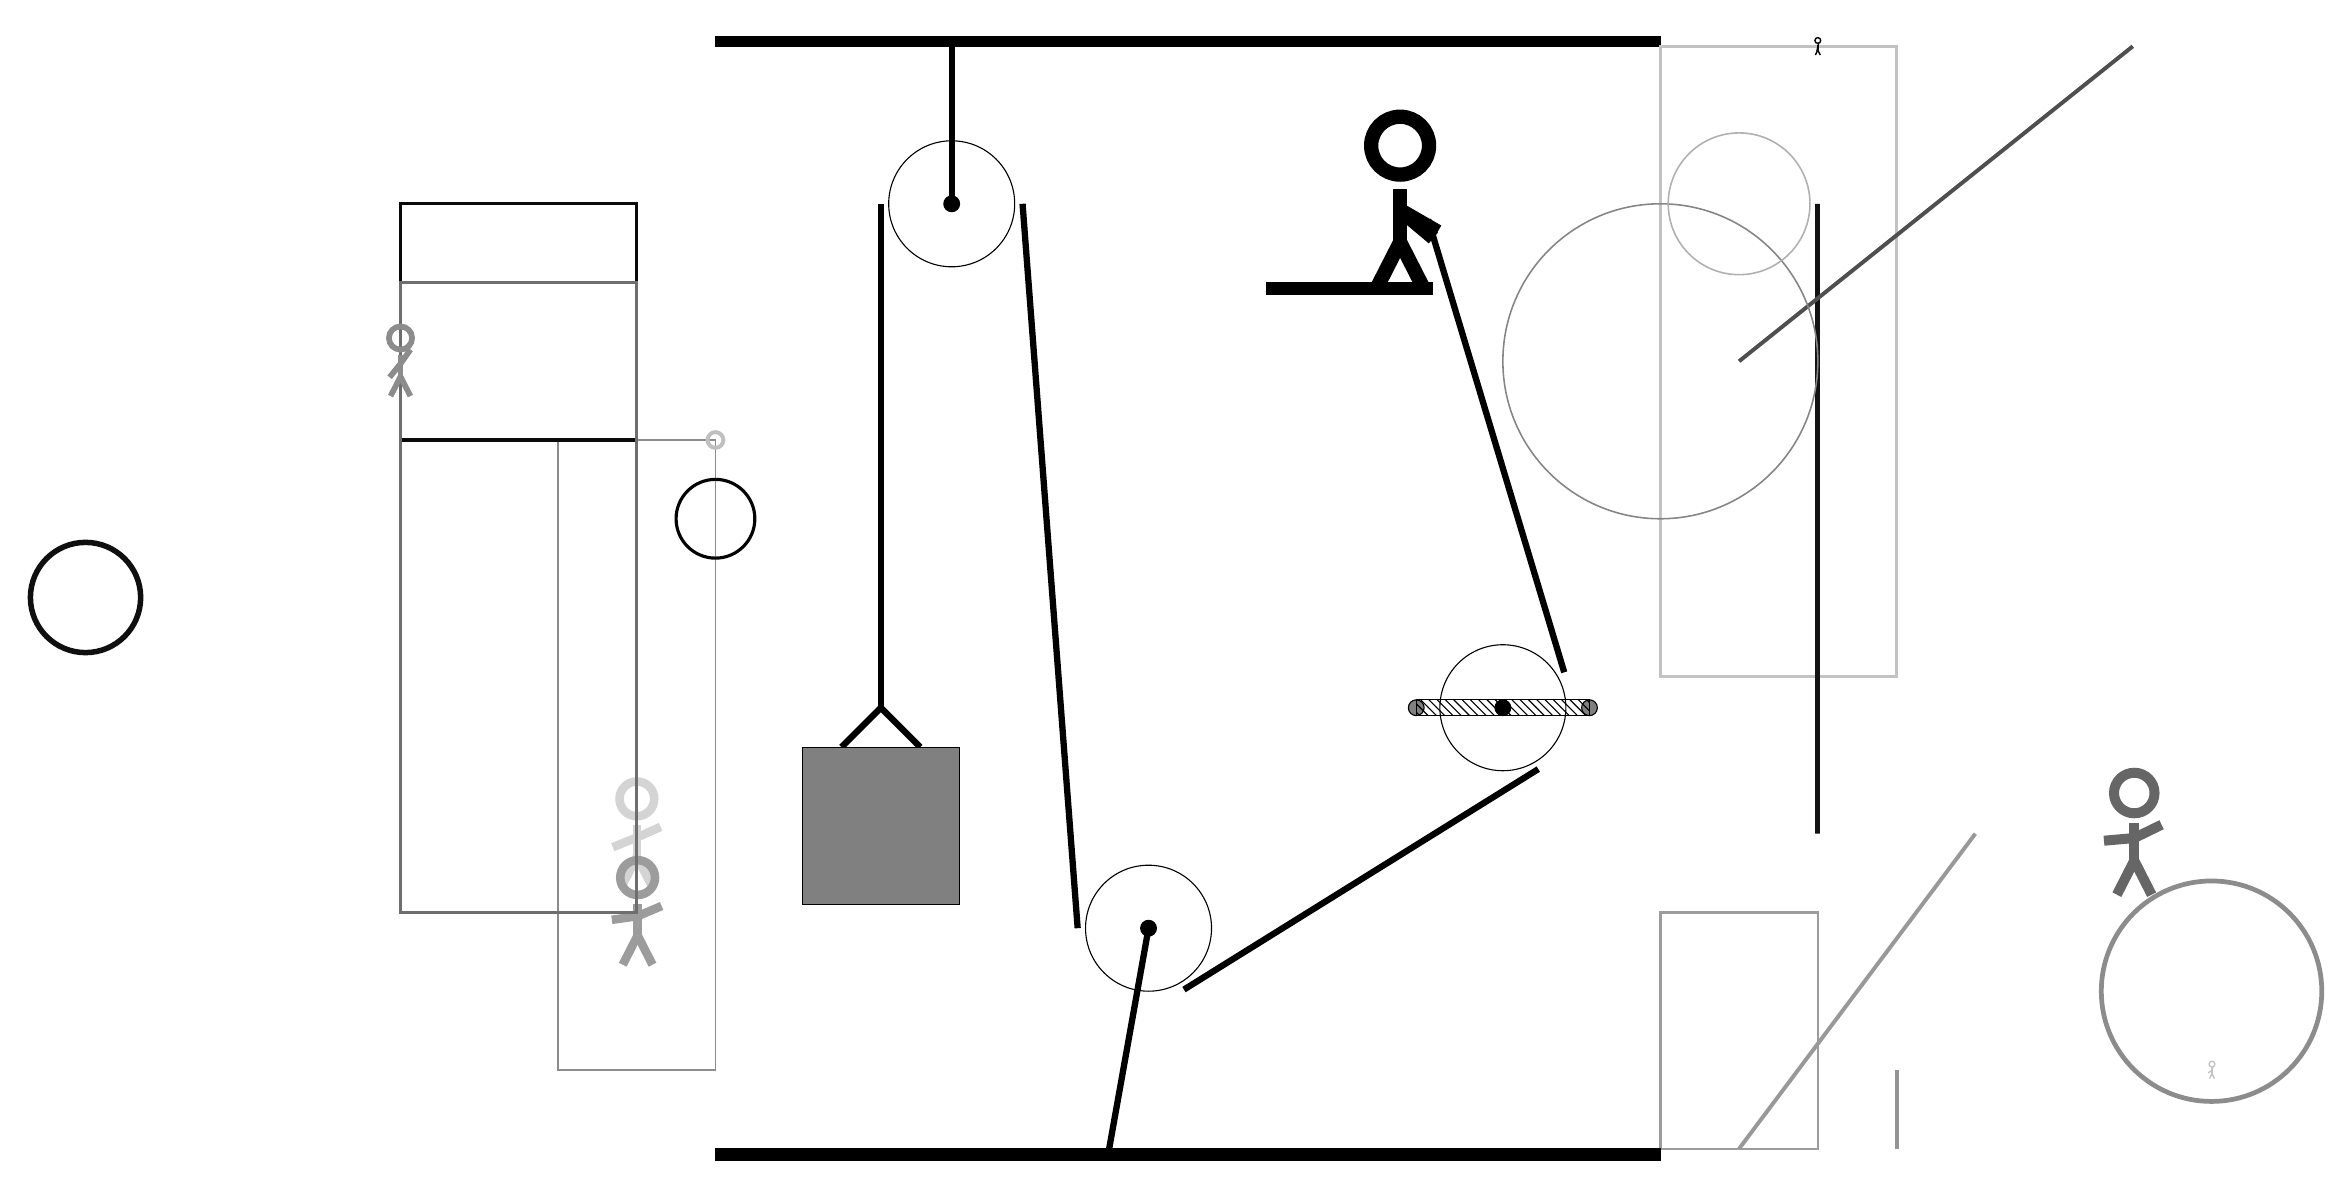
\begin{tikzpicture}
			%%%%% START %%%%%
			
			\draw[fill=black] (-2, 14) rectangle (10, 14.125);
			
			\draw (1, 12) circle (0.8);
			\draw[fill=black] (1, 12) circle (0.1);
			\draw[line width=0.8mm] (1, 14) -- (1, 12);
			
			\draw (3.5, 2.8) circle (0.8);
			\draw[fill=black] (3.5, 2.8) circle (0.1);
			\draw[line width=0.8mm] (3.5, 2.8) -- (3.0, 0);
			
			\draw[fill=white](8, 5.6) circle (0.8);
			\draw[fill=black] (8, 5.6) circle (0.1);
			\draw[fill=black!50] (9.1, 5.6) circle (0.1);
			\draw[fill=black!50] (6.9, 5.6) circle (0.1);
			\draw[pattern=north west lines, pattern color=black] (6.9, 5.7) rectangle (9.1, 5.5);
			
			\node[line width=0.3mm, color=black!17] at (-3, 4) {\Strichmaxerl[6][22][24]};
			
			\draw[line width=0.2mm, color=black!45] (-2, 1) rectangle (-4, 9);
			\node[line width=0.3mm, color=black!39] at (-3, 3) {\Strichmaxerl[6][8][23]};
			\draw[line width=0.4mm, color=black!24] (10, 6) rectangle (13, 14);
			\draw[line width=0.3mm, color=black!39] (12, 3) rectangle (10, 0);
			\draw[line width=0.6mm, color=black!93] (12, 4) rectangle (12, 12);
			\draw [line width=0.5mm, color=black!25](-2, 9) circle (0.1);
			\draw[line width=0.5mm, color=black!69](11, 10) -- (16, 14);
			\draw[line width=0.4mm, color=black!96] (-3, 9) rectangle (-6, 12);
			\draw [line width=0.2mm, color=black!48](10, 10) circle (2.0);
			
			\draw[line width=0.5mm, color=black!42](13, 0) -- (13, 1);
			\draw [line width=0.6mm, color=black!45](17, 2) circle (1.4);
			\node[line width=0.5mm, color=black!23] at (17, 1) {\Strichmaxerl[1][30][77]};
			
			\draw [line width=0.7mm, color=black!94](-10, 7) circle (0.7);
			\draw[line width=0.5mm, color=black!40](11, 0) -- (14, 4);
			\draw[line width=0.4mm, color=black!57] (-3, 3) rectangle (-6, 11);
			
			\draw [line width=0.2mm, color=black!31](11, 12) circle (0.9);
			\node[line width=0.7mm, color=black!60] at (16, 4) {\Strichmaxerl[7][5][26]};
			\node[line width=0.4mm, color=black!97] at (12, 14) {\Strichmaxerl[1][77][79]};
			\node[line width=0.2mm, color=black!45] at (-6, 10) {\Strichmaxerl[4][51][55]};
			\draw [line width=0.4mm, color=black!99](-2, 8) circle (0.5);
			
			\draw[line width=0.8mm](-0.4, 5.1) --  (0.1, 5.6) -- (0.6, 5.1);
			\draw[fill=black!50] (-0.9, 5.1) rectangle (1.1, 3.1);
			
			\draw[line width=0.8mm](0.1, 12) -- (0.1, 5.6);
			\centerarc[line width=0.8mm](1, 12)(180:0:0.9)
			\draw[line width=0.8mm](1.9, 12) -- (2.6, 2.8);
			\centerarc[line width=0.8mm](3.5, 2.8)(180:300:0.9);
			\draw[line width=0.8mm](3.95, 2.0206) -- (8.45, 4.8206);
			\centerarc[line width=0.8mm](8, 5.6)(300:390:0.9);
			\draw[line width=0.8mm](8.7794, 6.05) -- (7.05, 11.8);
			
			\node at (6.75, 12) {\Strichmaxerl[10][-220][-30]};
			\draw[fill=black] (5, 11) rectangle (7.1, 10.85);
			
			\draw[fill=black] (-2, 0) rectangle (10, -0.15);
			
			%%%%% END %%%%%
		\end{tikzpicture}
	\end{figure}	
\end{document}